\documentclass[10pt]{article}
\usepackage[
  paperheight=8.5in, 
  paperwidth=5.5in,
  margin=.5in
]{geometry}
\usepackage[per-mode=symbol]{siunitx}
\usepackage{tikz}
\usetikzlibrary{patterns,calc}
\tikzset{
  myaxis/.append style={
    ->,
    ultra thick
  },
  mygrid/.append style={
    dotted, thick
  },
  myminorgrid/.append style={
    dotted, thin
  },
  ball/.append style={
    shading=ball,
    minimum width=15pt
  },
  ground/.append style={
    pattern=north east lines
  },
  vel/.append style={
    ->,
    ultra thick,
    red
  },
  vellab/.append style={
    right=2pt,
  },
}



\begin{document}
\pagestyle{empty}





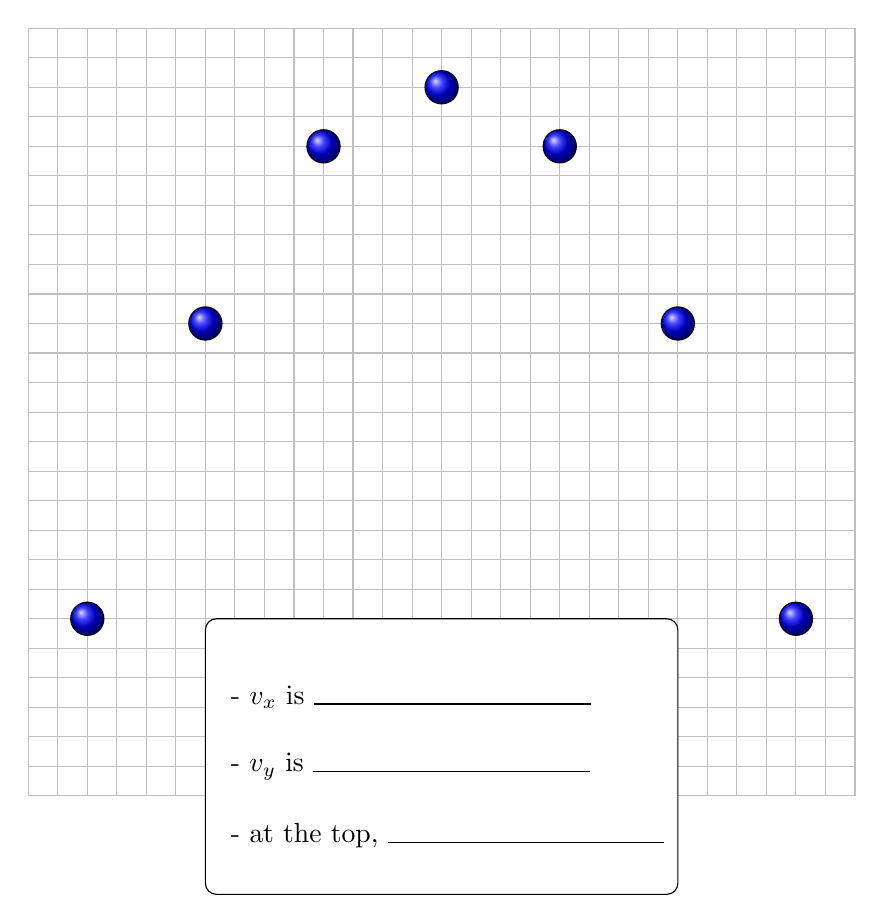
\begin{tikzpicture}
  \begin{scope}[every node/.append style={fill=white}]
    \def\scale{0.15}
    \def\xscale{1.5}
    \def\axisloc{-2}
    \def\velscale{.05}

    \draw[step=2.5*\scale, thin, gray!50] (-\xscale*0.5,-\scale*15) grid (\xscale*6.5,\scale*50);

    \draw[ball] (0,0) coordinate (a) 
      circle (6pt);
    \draw[ball] (\xscale*1,\scale*25) coordinate (b) 
      circle (6pt);
    \draw[ball] (\xscale*2,\scale*40) coordinate (c)
      circle (6pt);
    \draw[ball] (\xscale*3,\scale*45)  coordinate (d)
      circle (6pt);
    \draw[ball] (\xscale*4,\scale*40) coordinate (e)
      circle (6pt);
    \draw[ball] (\xscale*5,\scale*25) coordinate (f) 
      circle (6pt);
    \draw[ball] (\xscale*6,0) coordinate (g)
      circle (6pt);

    \draw[fill=white, rounded corners] (\xscale*1,0) rectangle (\xscale*5,-3.5);
    \draw (1.7,-1) node[anchor=west] {
        - $v_x$ is \rule{10em}{0.15mm}
      }
      ++ (0,-2.5em) node[anchor=west]  {
        - $v_y$ is \rule{10em}{0.15mm}
      }
      ++ (0,-2.5em) node[anchor=west]  {
        - at the top, \rule{10em}{0.15mm}
      };

  \end{scope}

\end{tikzpicture}


\vspace{1cm}

\paragraph{Consider these starting angles:}\hfill

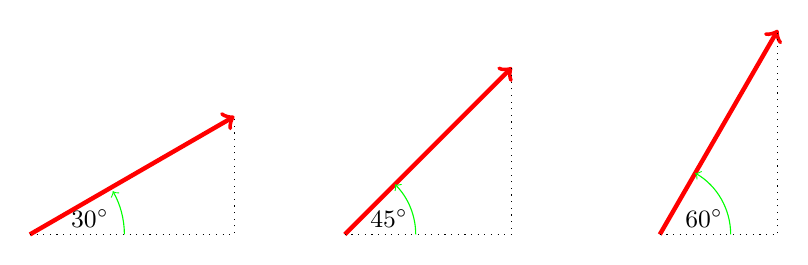
\begin{tikzpicture}
  \begin{scope}[
    vector/.append style={ultra thick,->,red},
    component/.append style={dotted},
    ang/.append style={->, green},
  ]
    \draw[vector] 
      (0,0) coordinate (a) -- ++(30:3) coordinate (b);
    \draw[component] (a) -| (b);
    \draw (a) ++ (.4,0.2) node[anchor=west] {\small $30^\circ$};
    \draw[ang] (a) ++ (1.2,0) arc (0:30:1.1);

    \draw[vector] 
      (4,0) coordinate (a) -- ++(45:3) coordinate (b);
    \draw[component] (a) -| (b);
    \draw (a) ++ (.2,0.2) node[anchor=west] {\small $45^\circ$};
    \draw[ang] (a) ++ (.9,0) arc (0:45:.9);

    \draw[vector] 
      (8,0) coordinate (a)-- ++(60:3) coordinate (b);
    \draw[component] (a) -| (b);
    \draw (a) ++ (.2,0.2) node[anchor=west] {\small $60^\circ$};
    \draw[ang] (a) ++ (.9,0) arc (0:60:.9);
  \end{scope}
\end{tikzpicture}





\end{document}